\documentclass[aspectratio=169]{beamer}
\usepackage[utf8]{inputenc}
\usepackage{hyperref}
\usepackage{amsmath,amsfonts,amsthm,bm}
\usepackage{color}
\usepackage{graphicx} % Allows including images
\usepackage{subcaption}
\usepackage{booktabs} % Allows the use of \toprule, \midrule and \bottomrule in tables
\usepackage{tikz}
\usepackage{color}
\usepackage{minted}
\usetikzlibrary{automata,positioning,shapes.geometric,shapes.misc,arrows}
%\usepackage{pgfplots}
\usepackage{listings}
\usepackage{courier}
\usepackage[version=4]{mhchem}
\usepackage{array}

\lstset{ %
    basicstyle=\scriptsize\ttfamily, % fonts that are used for the code
    breakatwhitespace=false,         % sets if automatic breaks should only happen at whitespace
%breaklines=true,                 % sets automatic line breaking
%captionpos=b,                    % sets the caption-position to bottom
    commentstyle=\color{gray}\textit,    % comment style
    keepspaces=true,                 % keeps spaces in text, useful for keeping indentation of code (possibly needs columns=flexible)
    keywordstyle=\color{blue},       % keyword style
    language=Python,                 % the language of the code
%otherkeywords={*,...},          % if you want to add more keywords to the set
    rulecolor=\color{black},         % if not set, the frame-color may be changed on line-breaks within not-black text (e.g. comments (green here))
    showspaces=false,                % show spaces everywhere adding particular underscores; it overrides 'showstringspaces'
    showstringspaces=false,          % underline spaces within strings only
    showtabs=false,                  % show tabs within strings adding particular underscores
    stringstyle=\color{red}, % string literal style
    tabsize=4,                       % sets default tabsize to 2 spaces
    columns=fixed                    % Using fixed column width (for e.g. nice alignment)
}

\hypersetup{
    colorlinks=true,
    linkcolor=red,
    filecolor=magenta,
    urlcolor=red,
}

\DeclareMathOperator*{\argmax}{argmax}
\DeclareMathOperator*{\argmin}{argmin}
\let \vec \mathbf

\newcommand{\classname}{NANO266}
\newcommand{\classyear}{Fall 2024}
\mode<presentation> {
    \usetheme{CambridgeUS}
    \setbeamertemplate{footline}[text line]{%
        \parbox{\linewidth}{\vspace*{-8pt}\classname\hfill\classyear\hfill\insertpagenumber}}

    %\setbeamertemplate{footline}[page number]
    \setbeamertemplate{navigation symbols}{}
}


\title[\classname Temperature]{\classname~- Quantum Mechanical Modeling of Materials and Nanostructures\\Temperature}

\author{Shyue Ping Ong}
\institute[UCSD]{University of California, San Diego\\
\medskip
}
\date{\classyear} % Date, can be changed to a custom date

\begin{document}


    \begin{frame}
        \titlepage % Print the title page as the first slide
    \end{frame}

\begin{frame}{What is Temperature?}
Temperature is a measure of ``excess'' energy above the ground state due to excitations.

\begin{figure}
    \centering
    \begin{subfigure}{0.45\textwidth}
        \centering
        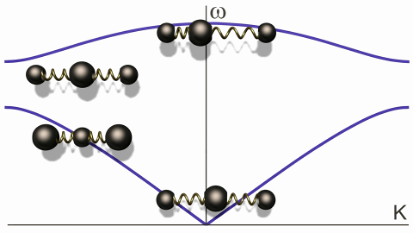
\includegraphics[width=0.5\linewidth]{figures/10_vibrational.png}
    \caption{Vibrational}
    \end{subfigure}
    \begin{subfigure}{0.45\textwidth}
        \centering
        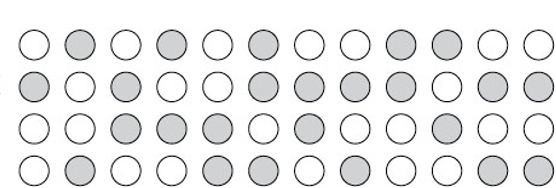
\includegraphics[width=0.7\linewidth]{figures/10_configurational.png}
    \caption{Configurational}
    \end{subfigure}
        \begin{subfigure}{0.45\textwidth}
        \centering
        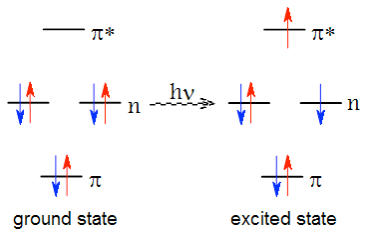
\includegraphics[width=0.5\linewidth]{figures/10_electronic.png}
    \caption{Electronic}
    \end{subfigure}
    \begin{subfigure}{0.45\textwidth}
        \centering
        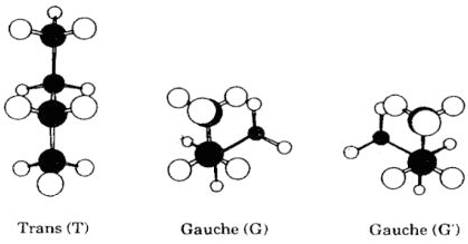
\includegraphics[width=0.7\linewidth]{figures/10_conformational.png}
    \caption{Conformational}
    \end{subfigure}
    \label{fig}
\end{figure} 

\end{frame} 

\begin{frame}{Approximating Temperature}
\begin{columns}
\column{0.5\textwidth}
Temperature changes oxygen chemical potential $\mu_{O_2}$:
\begin{eqnarray*}
\mu_{O_2}(T, p_{O_2}) & = & \mu_{O_2}(T, p_{O_2}^0)+ kT \ln \frac{p_{O_2}}{p_{O_2}^0}    
\end{eqnarray*} 

where $p_{O_2}$ is the partial pressure of oxygen.\newline
\newline 
For a reaction involving only solid phases and oxygen gas, the relevant thermodynanic potential is the grand potential:\cite{ongLiFeO22008}

\begin{eqnarray*}
    \phi & = & E - TS + PV - \mu_{O_2} N_{O_2}\\
    & \approx & E - \mu_{O_2} N_{O_2}
\end{eqnarray*}

\column{0.5\textwidth}

\begin{figure}
    \centering
    \begin{subfigure}{0.47\textwidth}
        \centering
        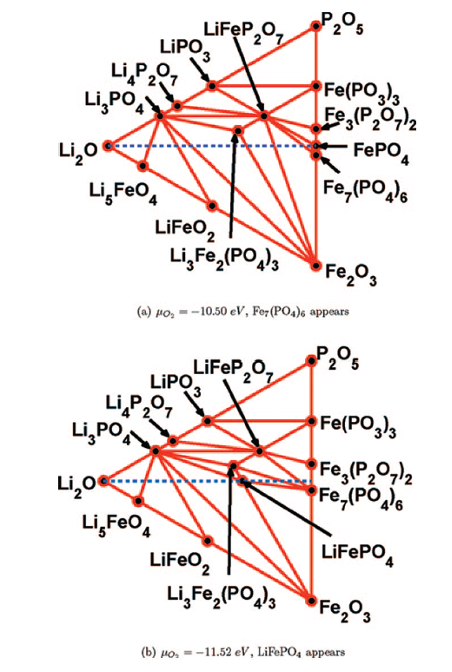
\includegraphics[width=\linewidth]{lectures/figures/10_LFP_PD.png}
    \end{subfigure}
    \begin{subfigure}{0.47\textwidth}
        \centering
        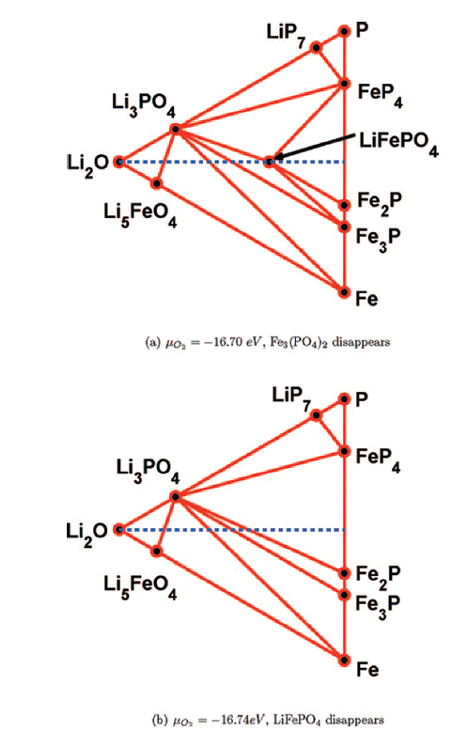
\includegraphics[width=\linewidth]{lectures/figures/10_LFP_PD2.png}
    \end{subfigure}
\end{figure} 
\end{columns} 
\end{frame} 

    \begin{frame}[allowframebreaks]{Bibliography}
        \bibliographystyle{unsrt}
        \bibliography{refs}
    \end{frame}



    \begin{frame}
        \Huge{\centerline{The End}}
    \end{frame}

\end{document}

